%%%%%%%%%%%%%%%%%%%%%%%%%%%%%%%%%%%%%%%%%%%%%%%%%%%%%%%%%%%%%%%%%%%%%%
%     File: ExtendedAbstract_intro.tex                               %
%     Tex Master: ExtendedAbstract.tex                               %
%                                                                    %
%     Author: Andre Calado Marta                                     %
%     Last modified : 27 Dez 2011                                    %
%%%%%%%%%%%%%%%%%%%%%%%%%%%%%%%%%%%%%%%%%%%%%%%%%%%%%%%%%%%%%%%%%%%%%%
% State the objectives of the work and provide an adequate background,
% avoiding a detailed literature survey or a summary of the results.
%%%%%%%%%%%%%%%%%%%%%%%%%%%%%%%%%%%%%%%%%%%%%%%%%%%%%%%%%%%%%%%%%%%%%%

\section{Introduction}
\label{sec:intro}

Planar materials have steadily been drawing the attention of the community since graphene was isolated from a graphite sample \cite{novoselov_electric_2004}.
Transition Metal Dichalcogenides (TMDs) are a class of such materials, appearing in the form of a variety of nanostructures.
Unlike in graphene, where the effects of electron interactions are relatively weak, in TMDs, electrons are strongly correlated, and one cannot overlook the interactions between them.
The increased complexity of the models describing such highly correlated materials, compared to their graphene counterparts, calls for sophisticated computer simulation methods, most notably Quantum Monte Carlo (QMC).

Much like graphite which is essentially constituted by stacked monolayers of carbon atoms bound by weak Van der Waals forces, 3D TMD structures are also formed by weakly bound layers.
However, instead of carbon, the layers contain transition metals $M$, and chalcogens $X$, in a $1-2$ proportion.
Thus, group 6 TMD are denoted $MX_2$, where $M = \text{Mo}, \text{W}, ...$ (respectively Molybdenum and Tungsten) and $X = \text{S}, \text{Se}, \text{Te}$ (respectively Sulfur, Selenium and Tellurium).
Each TMD monolayer contains a layer of $M$ atoms organized in a triangular lattice sandwiched between two layers of $X$ atoms,unlike graphene.
Each $M$ atom is coordinated with six $X$ atoms, in a stacked structure with various possible coordinations for the $X$ atoms.
The most common phases are trigonal prismatic (2H) and octahedral (1T), typically in the few $\angstrom$ range (for Molybdenum disulfide, $\text{Mo}\text{S}_2$, the width is around $6.5 \angstrom$).
Here we will consider the 2H configuration, whose planar honeycomb lattice is depicted in the top-down view of Fig (\ref{fig:tmdHex}a).
The valence bands arise out of the hybridization of the $d_{xy}$ and $d_{x^2 - y^2}$ orbitals of the transition metal with the $p_{x, y}$ orbitals of the chalcogen, while conduction bands have a main contribution from the $d_{3z^2 - r^2}$ orbitals of the $M$ atoms with only a minor contribution from the $p_{x, y}$ orbitals of the $X$ atoms.
\begin{figure}[H]
\centering
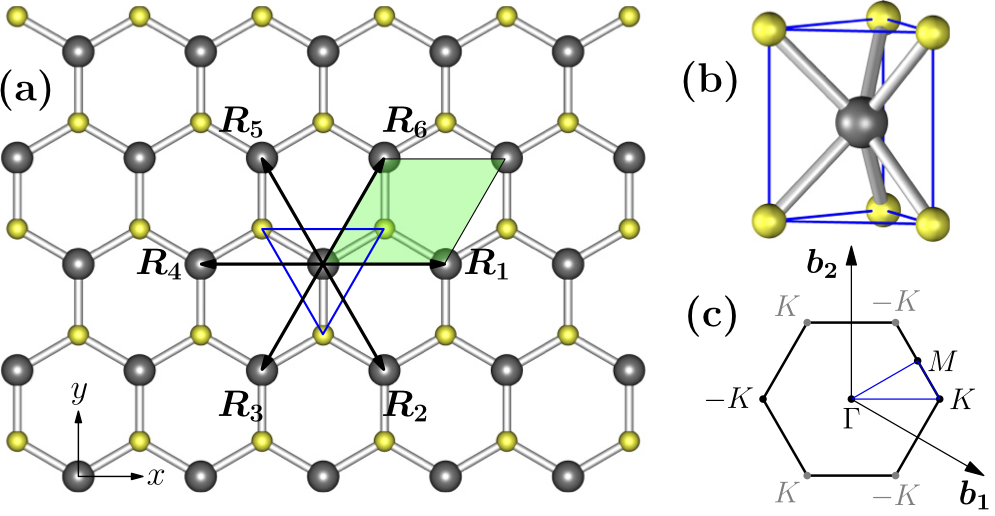
\includegraphics[width = 6cm]{images/tmd2.png}
 \caption{(a) M-coordination in the $2H$-phase of a TMD monolayer
(b) Unit cell of the $2H$-phase of a TMD monolayer.
(c) High symmetry points $\Gamma, M, K$ of the first Brillouin zone ($\bm b_{1,2}$ are the reciprocal basis vectors.(taken from \cite{liu_three-band_2013})}\label{fig:tmdHex}
\end{figure}